\begin{frame}
    \begin{figure}%
        \begin{tikzpicture}
        \only<1>{\node[anchor=south west,inner sep=0] (image) at (0,0) {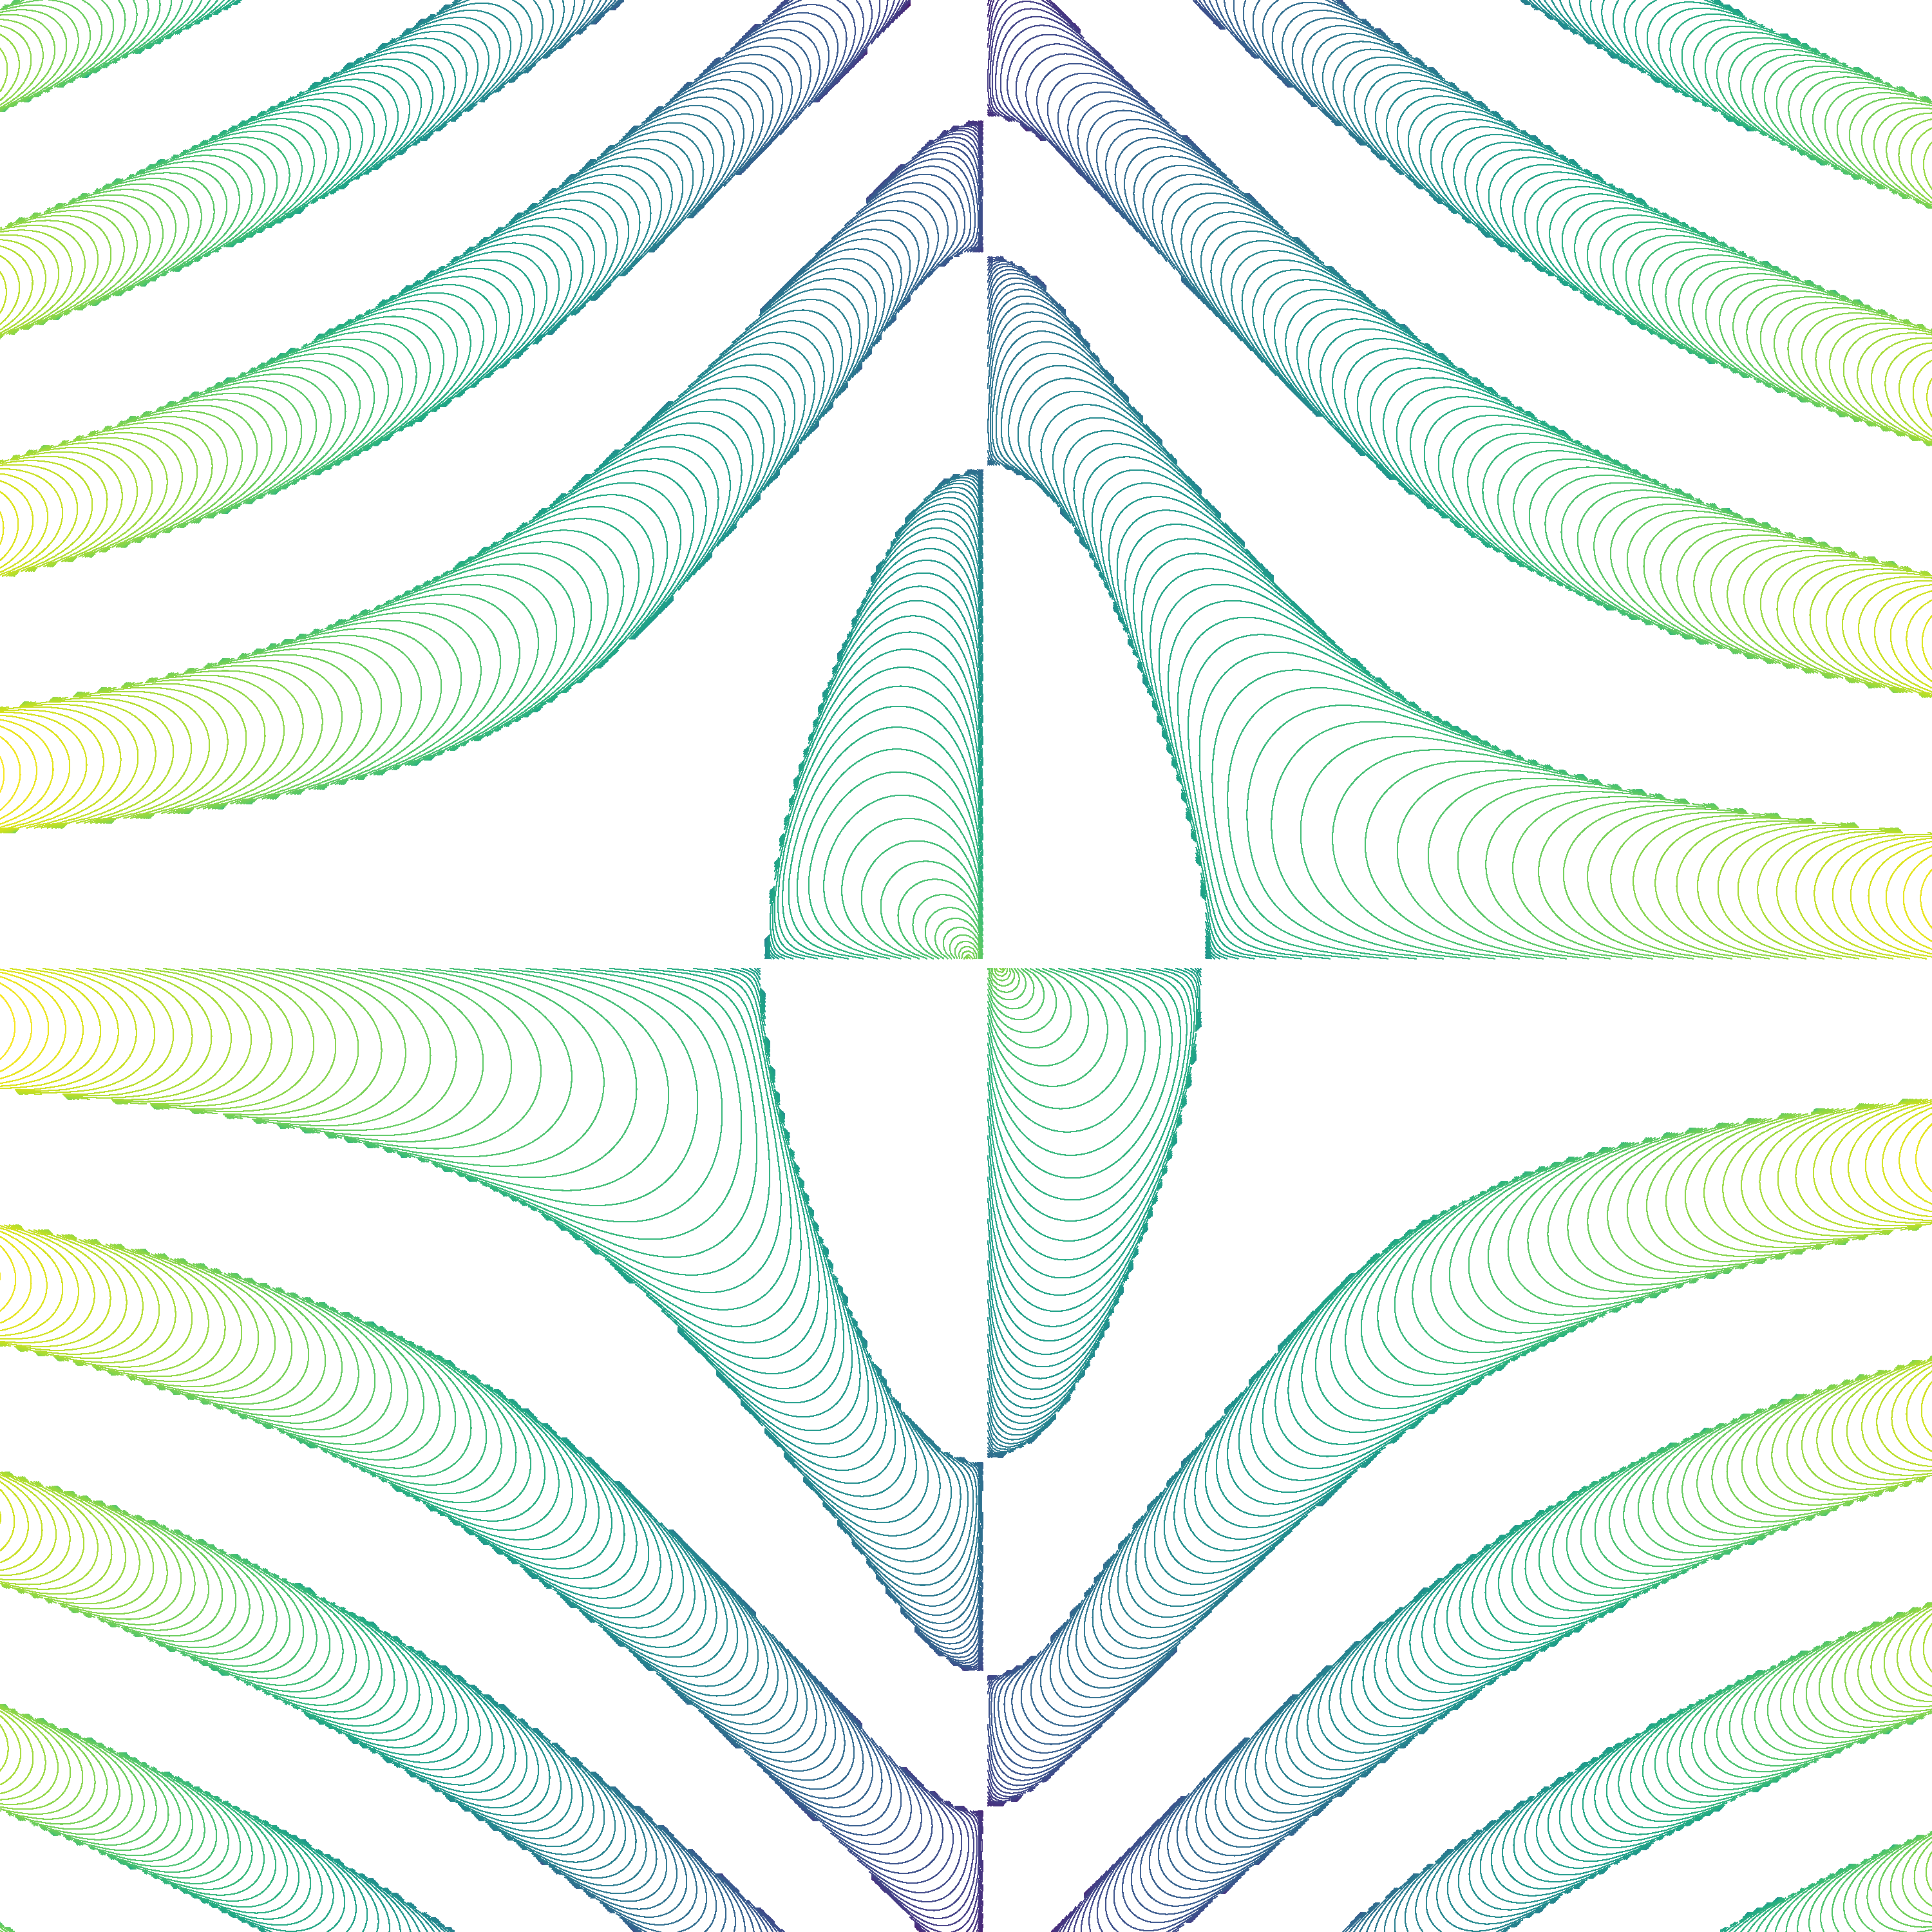
\includegraphics[width=0.55\textwidth]{figures/3030imag_contour_xi.pdf}};}
        \only<2>{\node[anchor=south west,inner sep=0] (image) at (0,0) {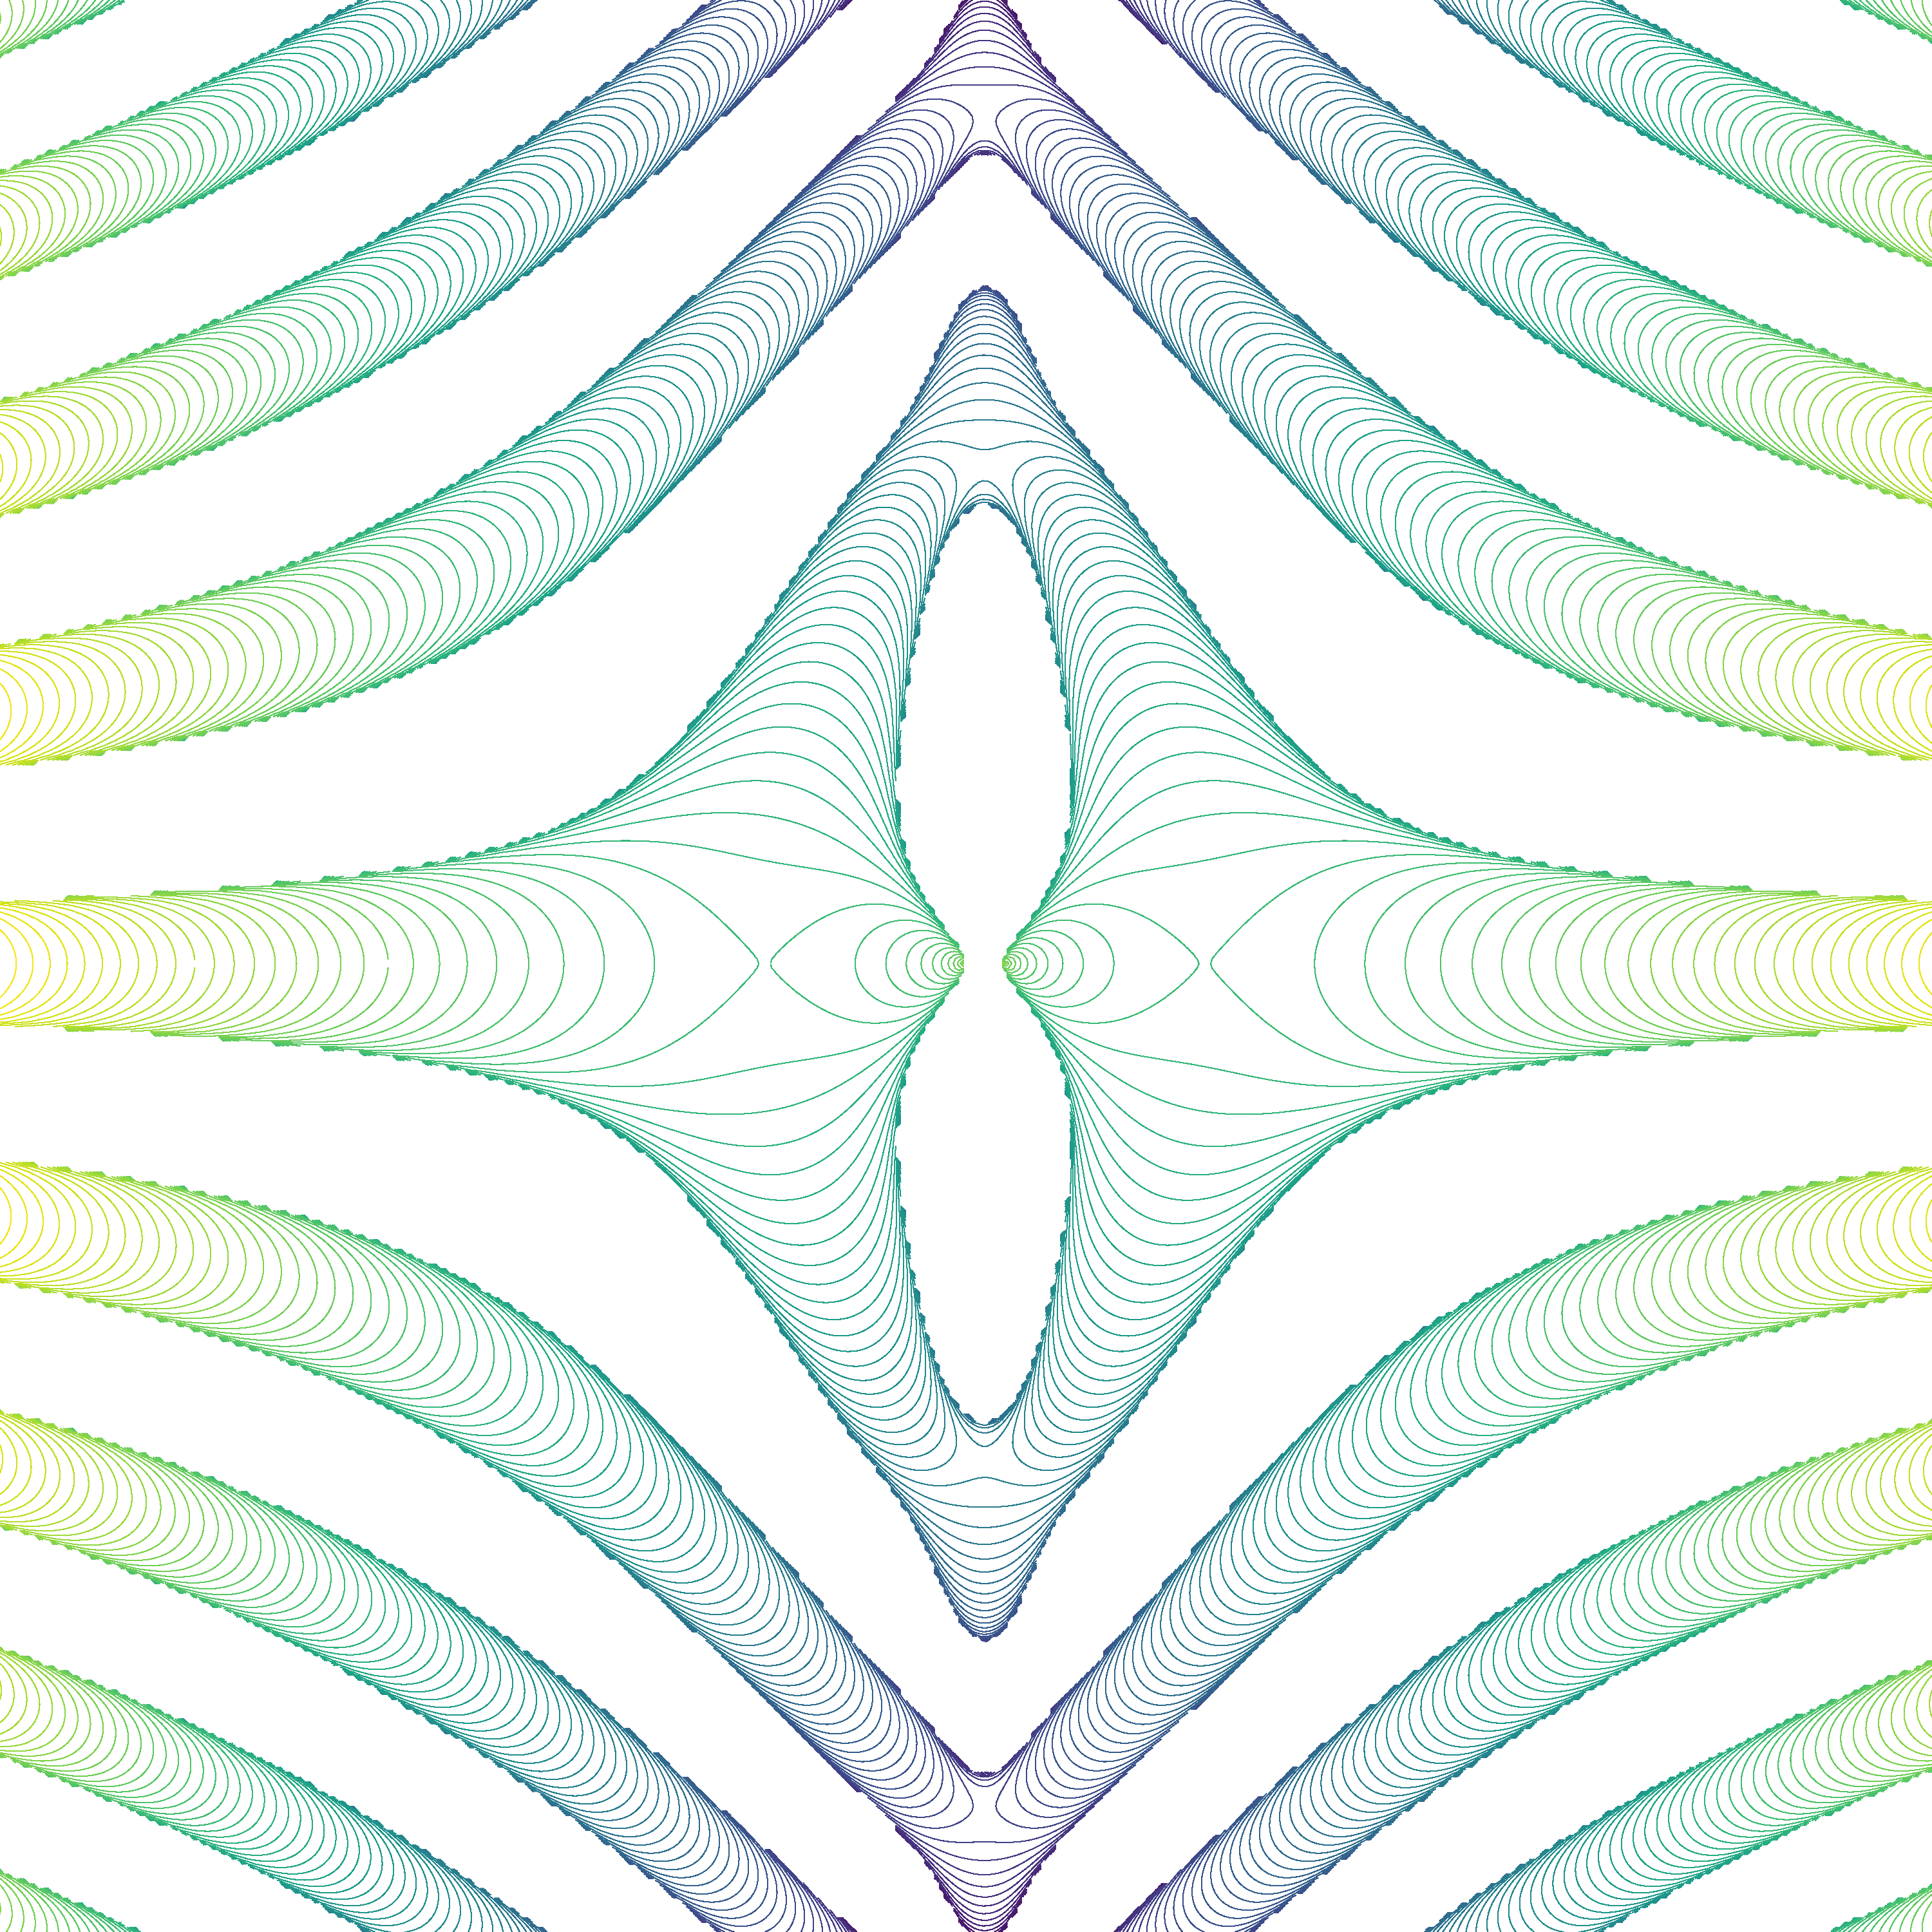
\includegraphics[width=0.55\textwidth]{figures/3030real_contour_xi.pdf}};}
        \only<3->{\node[anchor=south west,inner sep=0] (image) at (0,0) {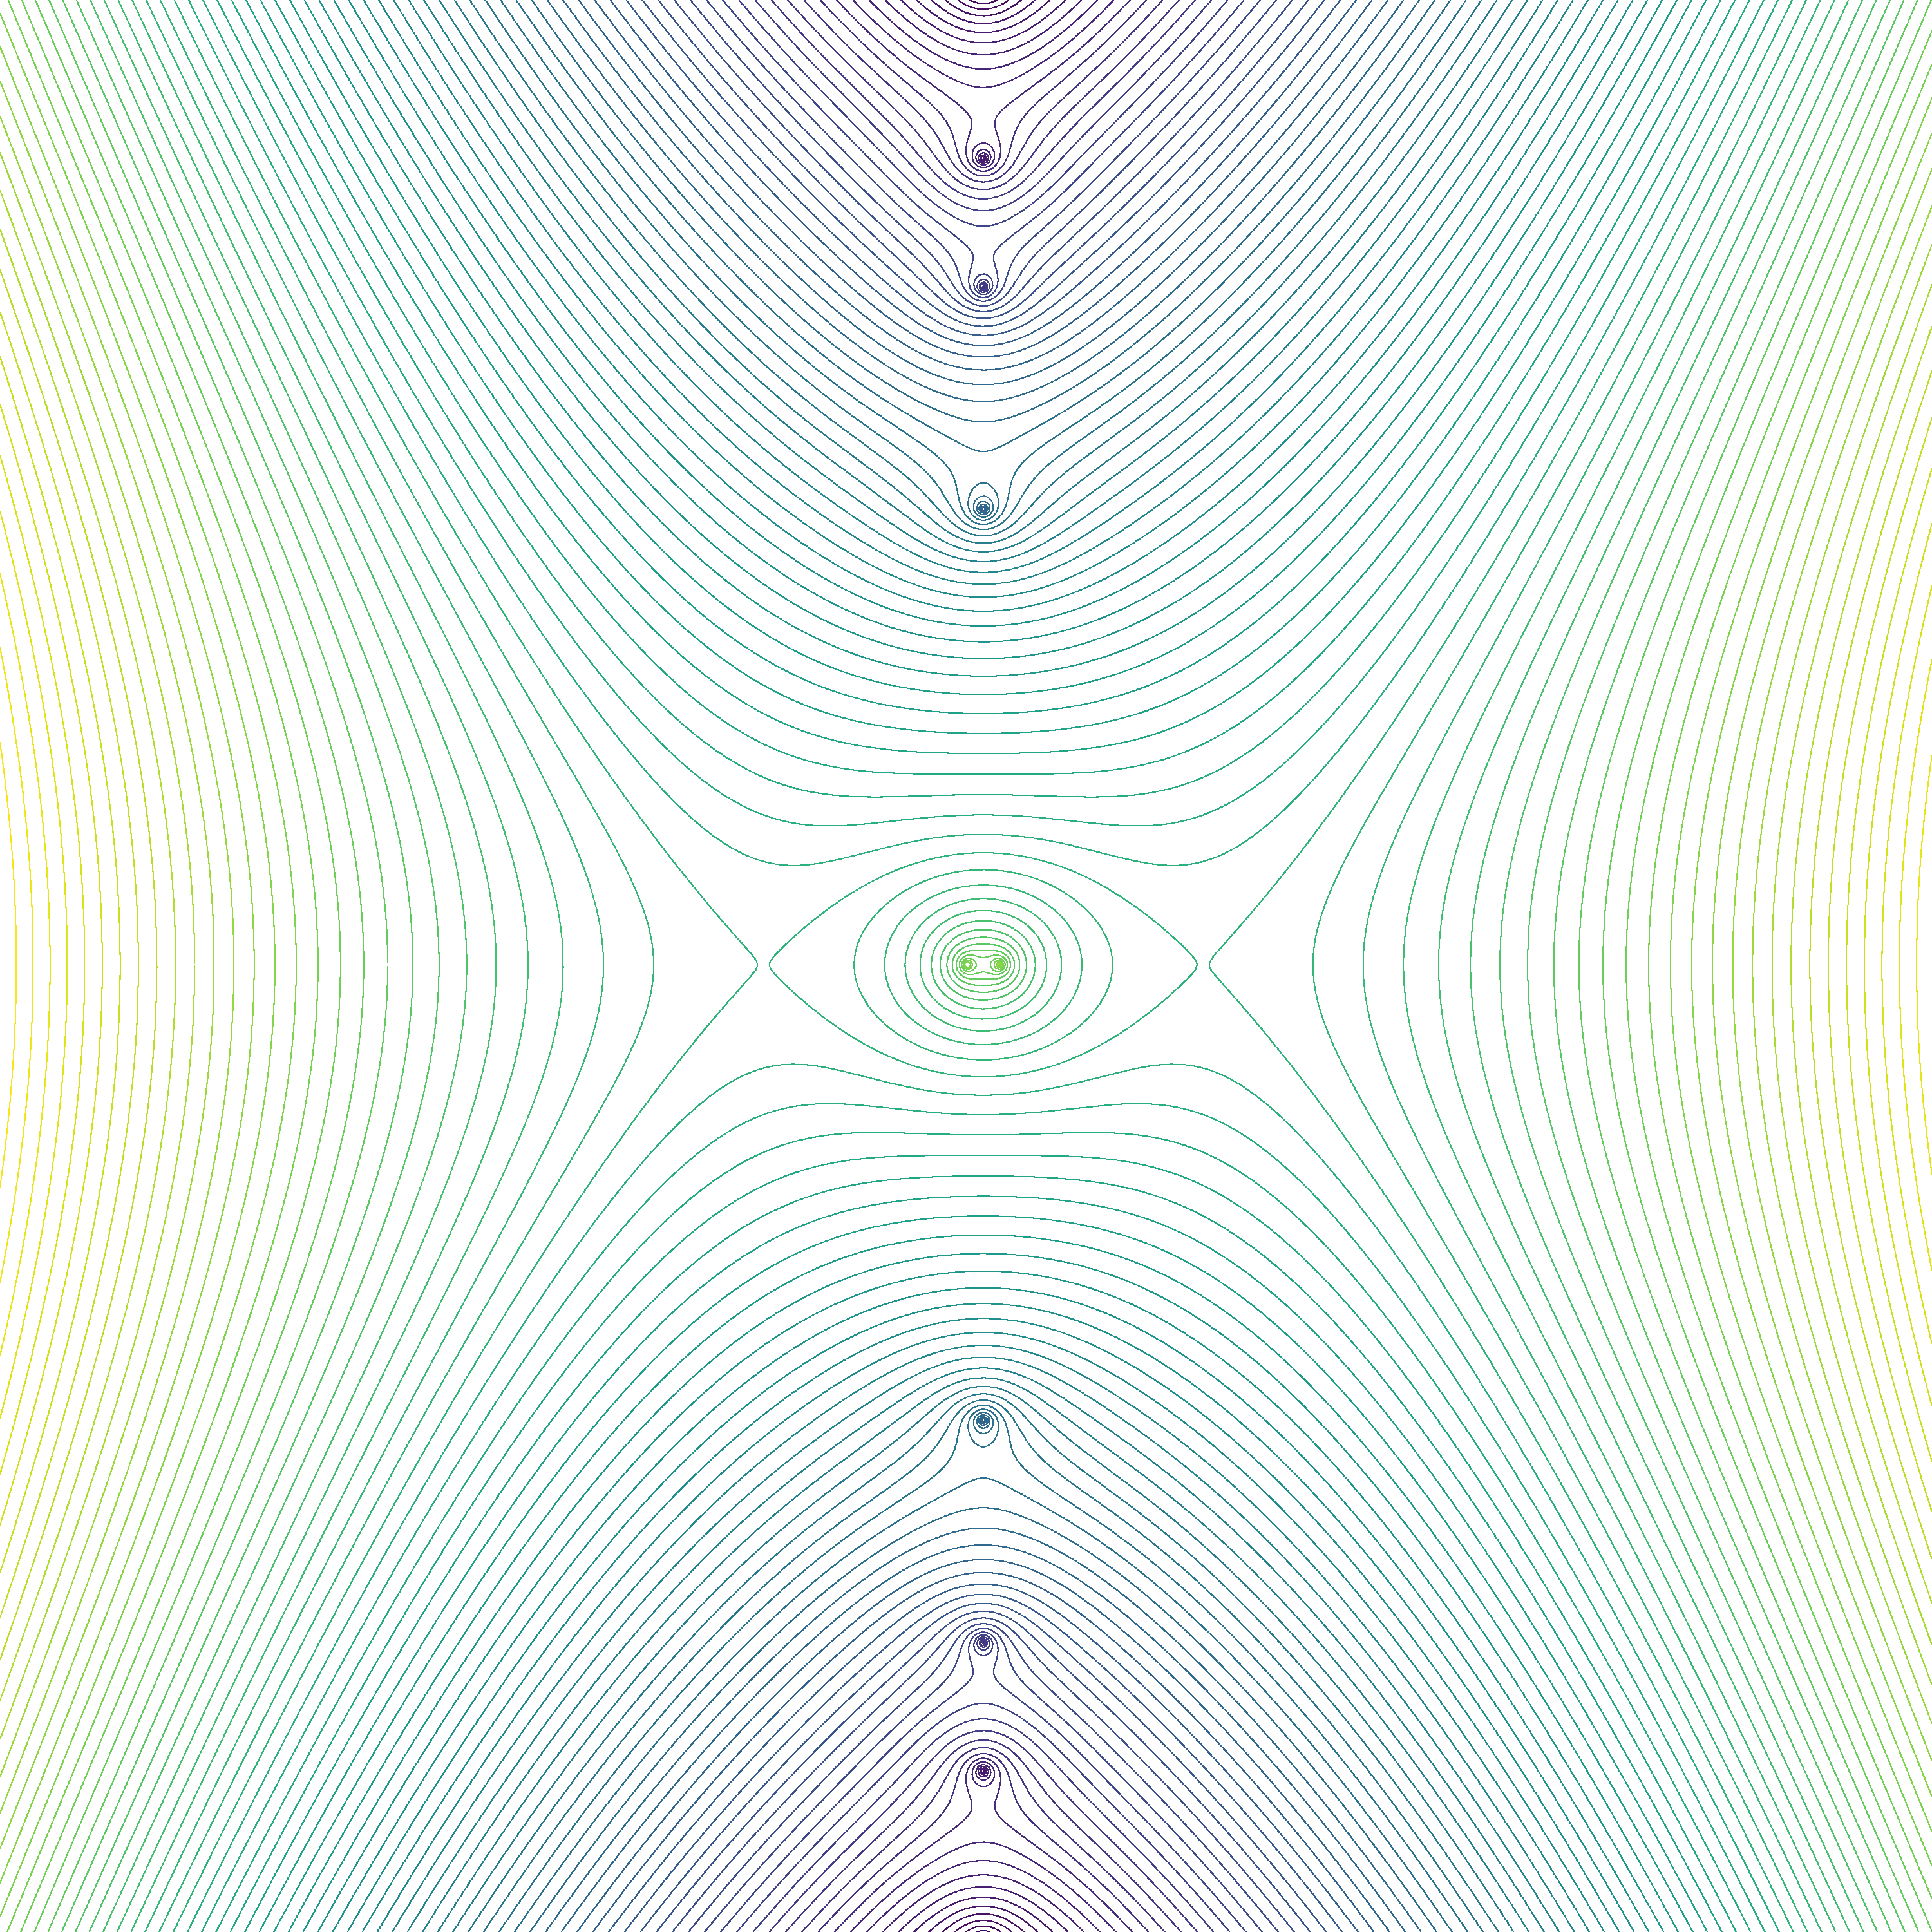
\includegraphics[width=0.55\textwidth]{figures/3030abs_contour_xi.pdf}};}
        \begin{scope}[x={(image.south east)},y={(image.north west)}]
            %\draw[help lines,xstep=.1,ystep=.1] (0,0) grid (1,1);
            \foreach \y in {-20,-10,...,20} {
                \node [anchor=east] at (0,\y/60+0.5) {$\y$}; 
                \draw (0,\y/60+0.5) -- (-1mm,\y/60+0.5);
                }
            \foreach \x in {-20,-10,0,1,10,20} { 
                \node [anchor=north] at (\x/56+0.5,0) {$\x$}; 
                \draw (\x/60+0.5,0) -- (\x/60+0.5,-1mm);
                }
            \node[rotate=90] (ylabel) at (-.12,0.5) {$\operatorname{\Im s}$};
            \node (xlabel) at (0.5,-.115) {$\operatorname{\Re s}$};
            \draw[very thin] (0,0) rectangle (1,1);
        \end{scope}
    \end{tikzpicture}%
    \vspace*{-13pt}
    \caption{\only<1>{Imaginärteil}\only<2>{Realteil}\only<3>{Betrag} der $\xi$-Funktion}
    \end{figure}
\end{frame}